\documentclass{article}
\usepackage{graphicx}
\usepackage{amsmath}
\usepackage[margin=3.5cm]{geometry}

\begin{document}

\title{Problem 17 - Arctangent function by numerical root finding}
\author{Jens S. K. Jensen}
\date{\today}
\maketitle

\section{Introduction}
This report covers a numerical implementation of the arctangent function
\begin{equation}
	a = arctan(x),
	\label{eq:atan1}
\end{equation}
by finding roots of the equation
\begin{equation}
	f(a) = tan(a) - x = 0.
	\label{eq:tan}
\end{equation}
That is, given $x$ find $a$ via eq. (\ref{eq:tan}).

\section{Implementation}
The numerical solution is implemented via a root-finding algorithm in GSL, in this case the \textit{gsl\_multiroot\_fdfsolver\_hybridsj} solver which relies on analytical derivatives, here
\begin{equation}
	\frac{d}{da}(tan(a) - x) = 1+tan(a)^2.
\end{equation}

The solver needs a starting point (henceforth called $a_0$), which if not chosen carefully can lead to undesirable results. All root-finding algorithms in the GSL multiroot library uses some variation of the newton iteration
\begin{equation}
	a_1 = a_0 - J(a_0)^{-1}f(a_0),
\end{equation}
with $a_0$ and $f(a_0)$ being vector quantities and $J(a_0)$ being the Jacobian matrix of the system. Looking at figure (\ref{fig:tan}) we see why we must choose $a_0$ with care. For instance, setting $a_0 = 0$ is fine for small values of $x$, but the algorithm will soon run rampant as $x$ exceeds $\pm \pi$ (for $a_0=0$), since the $arctan$ function only is defined for the initial repetition of the tangent function
\begin{equation}
	x = tan(a) \quad -\frac{\pi}{2}<a<\frac{\pi}{2}.
	\label{eq:limits}
\end{equation}

\begin{figure}[h]
	\centering
	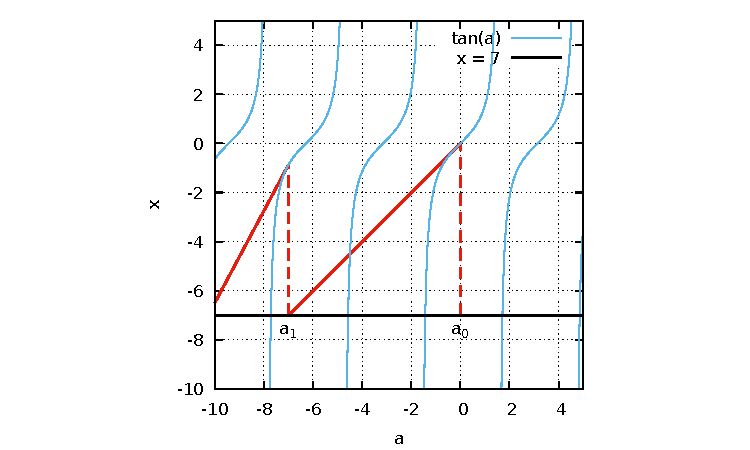
\includegraphics{tan.pdf}
	\caption{Progress of a Newton-Raphson algorithm starting with $a_0 = 0$ and $x = 7$}
	\label{fig:tan}
\end{figure}

Too alleviate this problem, the following definition for $a_0$ is made
\begin{equation}
	a_0 =
	\begin{cases}
		\dfrac{\pi}{2+1/x} \quad &\text{if} \quad x > 0 \\[10pt]
		-\dfrac{\pi}{2-1/x} \quad &\text{if} \quad x < 0 \\[10pt]
		0 \quad &\text{otherwise}
	\end{cases}
\end{equation}
This ensures that the algorithm will have a starting point that doesn't lead it beyond the limits in eq. (\ref{eq:limits}) (at least up to $x = \pm 100000$).

\section{Results}
The implemented numerical algorithm can be seen in figure (\ref{fig:atan}), along with the standard atan definition from the c library math.h.

\begin{figure}[h]
	\centering
	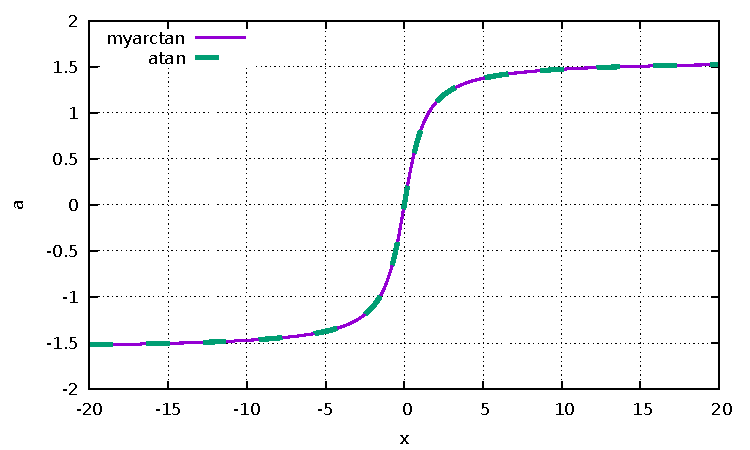
\includegraphics[width=0.67\textwidth]{atan.pdf}
	\caption{Visualization of the arctan function, showing both numerical implementation (myarctan) and the atan function from the math.h librabry}
	\label{fig:atan}
\end{figure}

\end{document}
